\chapter{Graph Coloring}

\providecommand{\degen}{\operatorname{degen}}

Hand someone a map of the counties of England and a box of crayons, and ask them
to color it so that no two counties sharing a border get the same color. They
will fumble for a minute, then settle into a rhythm, and they will never need
more than four colors. Reframe the map as a graph -- one vertex per county, an
edge between counties that touch -- and the puzzle becomes the central problem of
this chapter: assign a color to every vertex so that adjacent vertices differ,
using as few colors as you can. That number, the \emph{chromatic number}, is one
of the most studied and most stubborn quantities in all of graph theory.

Coloring is where graph theory stops being merely about reachability and starts
being about conflict. Edges no longer say ``you can get from here to there''; they
say ``these two things cannot be the same.'' Once you read an edge that way, a
flood of practical problems pours in. Registers in a compiler fight over a handful
of CPU slots; exams fight over a handful of time periods; radio transmitters fight
over a handful of frequencies. Every one of them is a coloring problem in
disguise, and every one of them inherits both the easy structure and the brutal
hardness that coloring carries.

This chapter builds the theory from the friendly end -- greedy bounds, bipartite
graphs, degeneracy -- up through two of the most elegant theorems in the subject,
Brooks's theorem on vertex coloring and Vizing's theorem on edge coloring. We then
visit the chordal and interval graphs, where coloring becomes straightforward and admits an
\emph{exact} linear-time solution by a one-pass greedy sweep, and we close by pointing at the
cliff edge: coloring a general graph optimally is NP-hard, and even approximating
it is hard. The applications -- register allocation and scheduling -- are not
afterthoughts; they are why the whole edifice was built.

\begin{historybox}
The modern subject of graph coloring originated with a simple cartographic observation.
In October 1852, Francis Guthrie, an undergraduate student at University College London,
was coloring a map of the counties of England. He noticed that four colors appeared to
suffice to color any map so that counties sharing a border segment received different
colors. Guthrie asked his brother Frederick, who consulted their professor Augustus De Morgan.
De Morgan posed the Four-Color Conjecture to Sir William Rowan Hamilton, who famously
dismissed it as uninteresting. The only mathematical tools available were Euler's polyhedral
formula ($V - E + F = 2$) and basic degree counting, which proved that every planar map must
contain at least one country with five or fewer neighbors.

In 1879, Alfred Kempe published a celebrated paper in the \emph{American Journal of Mathematics}
claiming to prove the Four-Color Conjecture. Kempe introduced \emph{Kempe chains}: alternating
two-colored paths that allow swapping colors locally to liberate a color for an uncolored
vertex. For eleven years, the mathematical community regarded the problem as solved.

In 1890, Percy Heawood uncovered a fatal flaw in Kempe's degree-$5$ case: swapping one
Kempe chain can inadvertently link or twist the boundaries of a second Kempe chain, causing
two neighbors to unexpectedly collide on the same color. While Kempe's proof fell apart,
Heawood salvaged his chains to prove the Five-Color Theorem.
Almost a century later, in 1976, Kenneth Appel and Wolfgang Haken at the University of
Illinois proved the Four-Color Theorem by reducing the problem to an unavoidable set of
$1{,}936$ reducible configurations checked by $1{,}200$ hours of computer calculations on an
IBM 370 mainframe. This ignited a passionate controversy across mathematics: can an argument
that cannot be verified by human hand with pencil and paper truly be accepted as a proof?
\end{historybox}

\chapterline

\section{Proper Colorings and the Chromatic Number}
\label{ch28:basics}

\begin{definition}[Proper coloring]
\label{ch28:def-coloring}
Let $\Gph=(V,E)$ be an undirected graph with no self-loops. A \emph{$k$-coloring}
is a function $c:V\to\set{1,2,\dots,k}$. It is \emph{proper} if $c(u)\neq c(v)$ for
every edge $uv\in E$. The graph is \emph{$k$-colorable} if a proper $k$-coloring
exists. The \emph{chromatic number} $\chi(\Gph)$ is the least $k$ for which $\Gph$
is $k$-colorable.
\end{definition}

The colors $1,\dots,k$ are just labels; nothing about them is ordered or numeric.
A proper $k$-coloring is the same data as a partition of $V$ into $k$ (possibly
empty) \emph{color classes} $V_1,\dots,V_k$, where each $V_i=c^{-1}(i)$ is an
\emph{independent set} -- a set of vertices with no edge inside it. So coloring is
exactly the problem of covering the vertex set by as few independent sets as
possible. We will lean on that dual view constantly: $\chi(\Gph)$ is the minimum
number of independent sets needed to partition $V$.

\begin{intuitionbox}
Three pictures to keep in your head. A path or any tree needs $2$ colors -- walk
along it flipping a switch. A triangle needs $3$: every pair of its vertices is
adjacent, so no two may share a color. And an odd cycle $C_{2k+1}$ needs $3$ even
though it looks like it ought to alternate: try to two-color it and the alternation
collides with itself when the cycle closes. The jump from ``looks alternating'' to
``actually needs three'' is the whole reason bipartiteness is special.
\end{intuitionbox}

A handful of exact values anchor intuition. The complete graph $K_n$ has every
pair adjacent, so all $n$ vertices need distinct colors and $\chi(K_n)=n$. A graph
with no edges has $\chi=1$. A cycle $C_n$ has $\chi(C_n)=2$ if $n$ is even and $3$
if $n$ is odd. Any tree with at least one edge has $\chi=2$.

\begin{figure}[H]
\centering
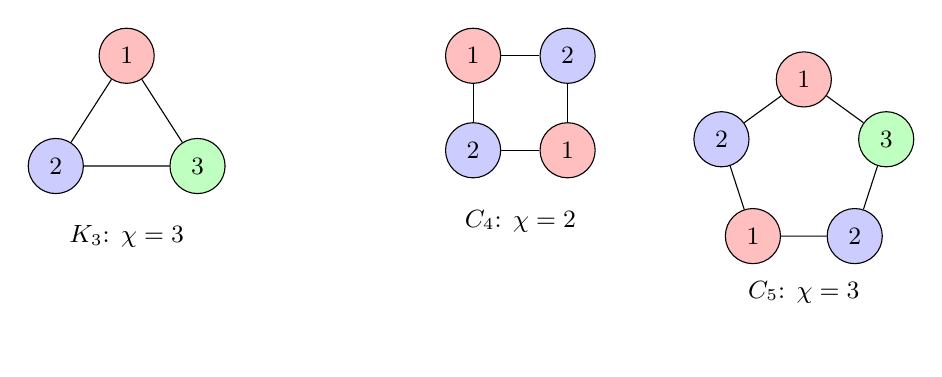
\begin{tikzpicture}[every node/.style={circle,draw,minimum size=7mm,inner sep=0pt,font=\small},
  c1/.style={fill=red!25}, c2/.style={fill=blue!20}, c3/.style={fill=green!25}]
% triangle
\begin{scope}[xshift=0cm]
  \node[c1] (a) at (0,1.4) {1};
  \node[c2] (b) at (-0.9,0) {2};
  \node[c3] (c) at (0.9,0) {3};
  \draw (a)--(b)--(c)--(a);
  \node[draw=none,fill=none] at (0,-0.9) {$K_3$: $\chi=3$};
\end{scope}
% even cycle C4
\begin{scope}[xshift=4.4cm]
  \node[c1] (p) at (0,1.4) {1};
  \node[c2] (q) at (1.2,1.4) {2};
  \node[c1] (r) at (1.2,0.2) {1};
  \node[c2] (s) at (0,0.2) {2};
  \draw (p)--(q)--(r)--(s)--(p);
  \node[draw=none,fill=none] at (0.6,-0.7) {$C_4$: $\chi=2$};
\end{scope}
% odd cycle C5
\begin{scope}[xshift=8.6cm]
  \node[c1] (1) at (90:1.1) {1};
  \node[c2] (2) at (162:1.1) {2};
  \node[c1] (3) at (234:1.1) {1};
  \node[c2] (4) at (306:1.1) {2};
  \node[c3] (5) at (18:1.1) {3};
  \draw (1)--(2)--(3)--(4)--(5)--(1);
  \node[draw=none,fill=none] at (0,-1.6) {$C_5$: $\chi=3$};
\end{scope}
\end{tikzpicture}
\caption{A triangle forces three colors; an even cycle alternates with two; an odd
cycle cannot alternate consistently and is forced up to three. The third color in
$C_5$ resolves the parity clash where the cycle closes.}
\label{ch28:fig-small}
\end{figure}

Two structural lower bounds fall out immediately and are worth naming because they
are the only general handles we get for free.

\begin{proposition}[Clique and independence-set bounds]
\label{ch28:prop-bounds}
For every graph $\Gph$ on $n$ vertices,
\[
  \omega(\Gph) \;\le\; \chi(\Gph) \;\le\; n,
  \qquad\text{and}\qquad
  \chi(\Gph)\;\ge\;\frac{n}{\alpha(\Gph)},
\]
where $\omega(\Gph)$ is the size of a largest clique and $\alpha(\Gph)$ the size
of a largest independent set.
\end{proposition}

\begin{proof}
A clique of size $\omega$ has all pairs adjacent, so its vertices receive
$\omega$ distinct colors; hence $\chi\ge\omega$. For the right inequality, color
all $n$ vertices distinctly. For the last bound: in a proper coloring each color
class is independent, so each has at most $\alpha$ vertices; $\chi$ classes cover
at most $\chi\cdot\alpha$ vertices, and this must be at least $n$.
\end{proof}

\begin{trapbox}
Do not mistake $\omega(\Gph)\le\chi(\Gph)$ for an equality. It is tempting because
it holds for many friendly graphs, but the gap can be arbitrarily large. The odd
cycle $C_5$ already shows it: $\omega(C_5)=2$ (no triangle) yet $\chi(C_5)=3$.
Worse, there exist \emph{triangle-free} graphs ($\omega=2$) with chromatic number
as large as you like -- Mycielski's construction builds them. Graphs where
$\omega=\chi$ holds for the graph \emph{and all its induced subgraphs} are exactly
the \emph{perfect graphs}, the subject of a later chapter; most graphs are not
perfect.
\end{trapbox}

\begin{historybox}
The word ``chromatic'' and the whole industry around it descend from the
\emph{Four Color Problem}: can every planar map be colored with four colors? Posed
by Francis Guthrie in 1852, it resisted proof for over a century, surviving a
famous flawed ``proof'' by Kempe in 1879 (whose chain-switching idea nonetheless
survives in modern algorithms). Appel and Haken finally settled it in 1976 with a
computer-assisted case analysis -- the first major theorem whose proof no human
could fully check by hand, and a philosophical lightning rod ever since. We treat
planarity in its own chapter; here we keep to general graphs.
\end{historybox}

\section{The Greedy Algorithm and Degeneracy}
\label{ch28:greedy}

The most basic coloring algorithm is the one a child uses: take the vertices in
some order, and give each the smallest color not already used by an
already-colored neighbor. It is myopic and it is not optimal, but it never fails to
produce a \emph{proper} coloring, and how many colors it spends depends entirely on
the order you feed it.

\begin{algorithm}[H]
\caption{\textsc{GreedyColor}$(\Gph, \pi)$ -- greedy coloring in a fixed order}
\label{ch28:alg-greedy}
\KwIn{Graph $\Gph=(V,E)$; an ordering $\pi=(v_1,\dots,v_n)$ of $V$.}
\KwOut{A proper coloring $c:V\to\set{1,2,\dots}$.}
\For{$i \leftarrow 1$ \KwTo $n$}{
  $S \leftarrow \set{\, c(u) : u \in N(v_i),\ u \text{ already colored}\,}$\;
  $c(v_i) \leftarrow$ smallest positive integer not in $S$\;
}
\Return $c$\;
\end{algorithm}

\begin{whybox}
Why is the output always proper? When we color $v_i$, we explicitly forbid every
color currently worn by a neighbor of $v_i$. A neighbor $v_j$ either is colored
already (we avoid its color now) or comes later (it will avoid \emph{our} color
when its turn arrives). Either way the edge $v_iv_j$ ends up bichromatic. So
correctness is free; the entire game is the \emph{number} of colors.
\end{whybox}

A clean upper bound comes from looking at how many \emph{earlier} neighbors each
vertex has.

\begin{proposition}[Greedy degree bound]
\label{ch28:prop-degree}
Running Algorithm~\ref{ch28:alg-greedy} uses at most $\Delta(\Gph)+1$ colors, where
$\Delta$ is the maximum degree. More sharply, if every vertex $v_i$ has at most $d$
neighbors among $v_1,\dots,v_{i-1}$ (its \emph{back-degree}), then at most $d+1$
colors are used.
\end{proposition}

\begin{proof}
When $v_i$ is colored, the forbidden set $S$ has size at most the number of
already-colored neighbors of $v_i$, which is its back-degree, $\le d$. The smallest
color avoiding a set of size $\le d$ is at most $d+1$. Since back-degree never
exceeds total degree $\le\Delta$, the global bound $\Delta+1$ follows.
\end{proof}

The sharper, back-degree version is the key to everything that follows, because it
says: \emph{we get to choose the order, so we should choose one that keeps
back-degrees small.} That motivates a graph parameter.

\begin{definition}[Degeneracy]
\label{ch28:def-degen}
A graph is \emph{$d$-degenerate} if every subgraph has a vertex of degree at most
$d$. The \emph{degeneracy} $\degen(\Gph)$ is the smallest such $d$.
\end{definition}

Equivalently, a graph is $d$-degenerate iff you can repeatedly delete a vertex of
degree $\le d$ until nothing is left. Reversing that deletion order gives an
ordering in which every vertex has back-degree $\le d$. This is the
\emph{degeneracy ordering}, and it is the order you want to hand the greedy
algorithm.

\begin{algorithm}[H]
\caption{\textsc{DegeneracyOrder}$(\Gph)$ -- smallest-last ordering}
\label{ch28:alg-degen}
\KwIn{Graph $\Gph=(V,E)$.}
\KwOut{Ordering $v_1,\dots,v_n$ with back-degrees $\le \degen(\Gph)$, and $d=\degen(\Gph)$.}
Maintain buckets $B_0,B_1,\dots$ where $B_j$ holds current vertices of residual degree $j$\;
$d \leftarrow 0$;\quad let $\mathrm{deg}[v]$ be the current degree of each $v$\;
\For{$i \leftarrow n,\,n-1,\,\dots,\,1$}{
  let $j^\star$ be the smallest nonempty bucket index; remove some $v$ from $B_{j^\star}$\;
  $d \leftarrow \max(d, j^\star)$;\quad $v_i \leftarrow v$\;
  \ForEach{still-present neighbor $u$ of $v$}{
    move $u$ from $B_{\mathrm{deg}[u]}$ to $B_{\mathrm{deg}[u]-1}$;\quad $\mathrm{deg}[u]\mathrel{-}=1$\;
  }
}
\Return $(v_1,\dots,v_n),\ d$\;
\end{algorithm}

\begin{whybox}
The smallest-last rule -- repeatedly peel off a minimum-degree vertex of the
\emph{current} graph and place it last -- realizes the degeneracy definition
directly. When vertex $v$ is peeled at residual degree $j^\star$, every vertex
remaining (which is exactly $v_1,\dots,v_{i-1}$) is an earlier vertex, so $v$'s
back-neighbors are precisely its still-present neighbors, of which there are
$j^\star\le d$. The maximum $j^\star$ over the whole peel is the degeneracy: it is
the largest minimum-degree you are ever forced to confront, which is exactly
$\max_{H\subseteq G}\delta(H)=\degen(\Gph)$. Using bucket lists, each edge is
touched a constant number of times, so the whole procedure runs in
$\Oh(n+m)$.
\end{whybox}

\begin{corollary}[Degeneracy coloring bound]
\label{ch28:cor-degen}
Every graph satisfies $\chi(\Gph)\le \degen(\Gph)+1$, and greedy coloring on the
degeneracy ordering achieves $\degen(\Gph)+1$ colors in $\Oh(n+m)$ time.
\end{corollary}

\begin{proof}
Order by Algorithm~\ref{ch28:alg-degen}; back-degrees are $\le\degen(\Gph)$; apply
Proposition~\ref{ch28:prop-degree}. The bucket peel is $\Oh(n+m)$, and a single greedy pass
where each vertex scans its earlier neighbors is also $\Oh(n+m)$ amortized.
\end{proof}

Degeneracy is sharper than $\Delta$ wherever the graph is locally dense but
globally sparse. A star $K_{1,n}$ has $\Delta=n$ but degeneracy $1$ (peel the
leaves), so $\chi\le 2$ -- correct. Planar graphs are $5$-degenerate, giving the
easy ``six-color theorem'' for planar maps in one line.

\begin{labbox}
Run greedy on the $4$-cycle $a$-$c$-$b$-$d$-$a$ (edges $ac,cb,bd,da$), which is
bipartite, so $\chi=2$. Two orders:
\begin{center}
\begin{tabular}{ll}
\toprule
Order $a,c,b,d$ & $c(a)=1$; $c$ adj $a\Rightarrow 2$; $b$ adj $c\Rightarrow 1$; $d$ adj $a,b\Rightarrow 2$. Two colors.\\
Order $a,b,c,d$ & $c(a)=1$; $b$ (not yet adj colored)$\Rightarrow 1$; $c$ adj $a,b\Rightarrow 2$; $d$ adj $a,b\Rightarrow 2$. Two colors.\\
\bottomrule
\end{tabular}
\end{center}
This $4$-cycle is too forgiving to expose greedy. The classic worst case is the
\emph{crown graph}: take $K_{n,n}$ minus a perfect matching; it is bipartite
($\chi=2$), yet the adversarial order $u_1,v_1,u_2,v_2,\dots$ forces greedy to use
$n$ colors. Build a small crown ($n=3$) by hand and watch greedy spiral: with the
matching $u_iv_i$ removed, $u_i$ joins every $v_j$ with $j\neq i$, so when greedy
hits $u_i$ (and then $v_i$) their already-colored neighbors are $v_1,\dots,v_{i-1}$
(respectively $u_1,\dots,u_{i-1}$), carrying colors $1,\dots,i-1$, and the pair $u_i,v_i$
takes a fresh color $i$. The lesson:
greedy's color count is an ordering artifact, never an invariant of the graph.
\begin{center}
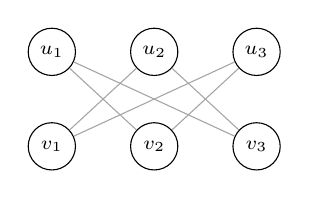
\begin{tikzpicture}[every node/.style={circle,draw,minimum size=6mm,inner sep=0pt,font=\scriptsize}]
  \foreach \i in {1,2,3}{
    \node (u\i) at (\i*1.3,1.2) {$u_\i$};
    \node (v\i) at (\i*1.3,0)   {$v_\i$};
  }
  % edges: u_i to v_j for i != j
  \foreach \i in {1,2,3}\foreach \j in {1,2,3}{
    \ifnum\i=\j\else \draw[gray!70] (u\i)--(v\j);\fi
  }
\end{tikzpicture}
\end{center}
The crown $S_3^0$: each $u_i$ misses only its partner $v_i$. Feeding greedy the order
$u_1,v_1,u_2,v_2,u_3,v_3$ paints all three $v_i$ different colors.
\end{labbox}

\begin{trapbox}
There \emph{always} exists an ordering on which greedy uses exactly $\chi(\Gph)$
colors -- take any optimal coloring and list color class $1$ first, then class $2$,
and so on. So greedy is ``optimal with the right order.'' This is useless
algorithmically: finding that order is as hard as coloring itself. Never conclude
from ``greedy can be optimal'' that ``greedy is good''; the missing piece is the
order, and the order hides all the difficulty.
\end{trapbox}

\section{Bipartite Graphs: Two Colors and a Certificate}
\label{ch28:bipartite}

The cleanest island of tractability is $\chi\le 2$. A graph is $2$-colorable
exactly when it is \emph{bipartite}, and there is a perfect, checkable obstruction:
the odd cycle.

\begin{theorem}[Konig's characterization]
\label{ch28:thm-bipartite}
For a graph $\Gph$ the following are equivalent:
\begin{enumerate}[label=\textup{(\arabic*)}]
  \item $\chi(\Gph)\le 2$;
  \item $\Gph$ is bipartite (its vertices split into two independent sets);
  \item $\Gph$ contains no cycle of odd length.
\end{enumerate}
\end{theorem}

\begin{proof}
(1)$\Leftrightarrow$(2) is the definition of a $2$-coloring read as a bipartition.
For (2)$\Rightarrow$(3): in a bipartition $(X,Y)$ every edge crosses, so any closed
walk alternates sides and must have even length; an odd cycle is an odd closed walk
and cannot exist. For (3)$\Rightarrow$(2): assume $\Gph$ connected (otherwise treat
components separately). Pick a root $r$, run BFS, and color $v$ by the parity of its
distance $\dist(r,v)$: even $\to X$, odd $\to Y$. Suppose some edge $uv$ joins two
vertices of equal parity. The tree paths $r\!\to\!u$ and $r\!\to\!v$ together with
edge $uv$ form a closed walk of length $\dist(r,u)+\dist(r,v)+1$, which is odd; a
standard argument extracts an odd cycle from any odd closed walk, contradicting
(3). So every edge crosses the bipartition.
\end{proof}

The proof is constructive: BFS two-colors a bipartite graph and, when it fails,
hands back an odd cycle as a \emph{certificate} of non-bipartiteness. That
certificate is what makes ``is this $2$-colorable?'' decidable in linear time, in
sharp contrast to ``is this $3$-colorable?'', which we will see is NP-complete.

\begin{algorithm}[H]
\caption{\textsc{TwoColor}$(\Gph)$ -- BFS bipartiteness test and coloring}
\label{ch28:alg-twocolor}
\KwIn{Connected graph $\Gph=(V,E)$.}
\KwOut{A proper $2$-coloring, or an odd cycle.}
$c[v]\leftarrow \bot$ for all $v$; pick a start $s$; $c[s]\leftarrow 0$; queue $Q\leftarrow\set{s}$\;
\While{$Q$ nonempty}{
  $u\leftarrow$ dequeue $Q$\;
  \ForEach{neighbor $w$ of $u$}{
    \uIf{$c[w]=\bot$}{$c[w]\leftarrow 1-c[u]$; enqueue $w$\;}
    \ElseIf{$c[w]=c[u]$}{\Return odd cycle through $u,w$ via BFS-tree paths\;}
  }
}
\Return coloring $c$\;
\end{algorithm}

\begin{complexitybox}
\textsc{TwoColor} is one BFS: $\Oh(n+m)$ time, $\Oh(n)$ space. It both decides
bipartiteness and produces a witness in either direction -- a $2$-coloring or an
odd cycle. This is the gold standard a coloring algorithm aspires to and almost
never achieves beyond two colors.
\end{complexitybox}

\begin{connectionbox}
Bipartite graphs are where coloring, matching, and flow all meet. Konig's theorem
(this one) is the coloring face of \emph{Konig's matching theorem} -- in a
bipartite graph the maximum matching equals the minimum vertex cover -- which the
matching chapter proves via flow. The two-coloring is also a spectral fingerprint:
a connected bipartite graph is precisely one whose largest \emph{adjacency}
eigenvalue $\lambda_{\max}$ is matched by $-\lambda_{\max}$ as the smallest, and
whose Laplacian spectrum has a corresponding symmetry. Two-colorability is the most
elementary spectral signature a graph carries, taken up in the spectral chapters.
\end{connectionbox}

\section{Brooks's Theorem}
\label{ch28:brooks}

The bound $\chi\le\Delta+1$ from greedy is tight -- complete graphs and odd cycles
hit it. Brooks's theorem says those two families are the \emph{only} obstructions:
for everything else you can shave one color off.

\begin{theorem}[Brooks, 1941]
\label{ch28:thm-brooks}
Let $\Gph$ be a connected graph with maximum degree $\Delta$. Then
$\chi(\Gph)\le\Delta$ unless $\Gph$ is a complete graph $K_{\Delta+1}$ or an odd
cycle, in which case $\chi(\Gph)=\Delta+1$.
\end{theorem}

\begin{intuitionbox}
Why should removing the two exceptional families buy a color? Greedy spends
$\Delta+1$ only if some vertex sees all $\Delta$ colors already used among its
neighbors at the moment it is colored. If we could always arrange that \emph{at
least two} neighbors of the troublesome last vertex already share a color -- so the
neighbors waste a color on a repeat -- then $\Delta$ colors suffice. The proof
engineers exactly such an ordering, and the only graphs where no such arrangement
exists are the rigid ones: cliques (every neighbor pair is adjacent, no repeats
possible) and odd cycles (too thin to create a repeat).
\end{intuitionbox}

We give the clean ordering-based proof for the main case.

\begin{proof}[Proof (main case)]
Assume $\Gph$ is connected, not complete, not an odd cycle, with $\Delta\ge 3$.
(The cases $\Delta\le 2$ are direct: $\Delta=0,1$ are trivial, and a connected
$\Delta=2$ graph is a path or a cycle, where only odd cycles need $3$ colors.)

\textbf{Case A: $\Gph$ is not $\Delta$-regular.} Then some vertex $v_n$ has degree
$<\Delta$. Build a BFS tree rooted at $v_n$ and order the vertices in
\emph{decreasing} BFS depth, breaking ties arbitrarily, so $v_n$ comes last. Every
$v_i$ with $i<n$ has at least one neighbor strictly closer to $v_n$ (its BFS parent),
which comes \emph{later} in this order; hence $v_i$'s back-degree is at most
$\deg(v_i)-1\le\Delta-1$. And $v_n$ itself has degree $<\Delta$. Greedy in this
order never sees $\Delta$ forbidden colors, so it uses $\le\Delta$.

\textbf{Case B: $\Gph$ is $\Delta$-regular.} Here every vertex has exactly $\Delta$
neighbors, so the parent trick alone leaves the last vertex exposed. The fix is to
plant a deliberate color repeat. One can show that a connected, $\Delta$-regular,
non-complete graph with $\Delta\ge3$ contains a vertex $v_n$ with two non-adjacent
neighbors $a=v_1$ and $b=v_2$ such that $\Gph-\set{a,b}$ stays connected. (If
$\Gph$ is $2$-connected this is a short argument; if it has a cut vertex one
descends into the blocks and inducts.) Order $v_3,\dots,v_{n-1}$ by decreasing BFS
depth from $v_n$ inside $\Gph-\set{a,b}$, ending with $v_n$.

Now run greedy. Give $a$ and $b$ the same color $1$ (legal, they are non-adjacent).
Every internal $v_i$ ($3\le i\le n-1$) has a later neighbor toward $v_n$, hence
back-degree $\le\Delta-1$, so $\le\Delta$ colors suffice for it. Finally $v_n$ has
$\Delta$ neighbors, but two of them, $a$ and $b$, share color $1$; so $v_n$'s
neighbors wear at most $\Delta-1$ distinct colors, and a free color in
$\set{1,\dots,\Delta}$ remains. Thus $\chi(\Gph)\le\Delta$.
\end{proof}

\begin{trapbox}
The delicate clause is ``find $v_n$ with two non-adjacent neighbors keeping
$\Gph-\set{a,b}$ connected.'' If you skip the connectivity requirement, the
decreasing-depth ordering can strand some vertex with all $\Delta$ neighbors
earlier, and the saved color evaporates. The full proof must also rule out the case
where every two neighbors of every vertex are adjacent -- but that forces a clique
on each neighborhood, and a connected such graph is itself complete, already
excluded. This neighborhood-clique trap is exactly where Kempe's 1879 four-color
``proof'' went wrong in spirit: an unjustified assumption that a convenient local
configuration always exists.
\end{trapbox}

\begin{historybox}
R.~Leonard Brooks proved this in 1941 while a student, in a circle that included
Smith, Stone, and Tutte -- the quartet famous for ``squaring the square.'' The
theorem is a rare instance where the worst case of a greedy bound is completely
characterized: two infinite families and nothing else. Lovasz later gave a slick
proof via ordering and a recoloring lemma; the argument above is in that lineage.
\end{historybox}

\section{Edge Coloring and Vizing's Theorem}
\label{ch28:vizing}

Shift attention from vertices to edges. An \emph{edge coloring} assigns colors to
edges so that edges sharing an endpoint differ; the minimum number of colors is the
\emph{chromatic index} $\chi'(\Gph)$. The model is scheduling matches in a
tournament: edges meeting at a vertex are games involving the same player and
cannot run at the same time, so each color is a round of simultaneous,
non-conflicting games.

\begin{intuitionbox}
Edge coloring of $\Gph$ is exactly vertex coloring of its \emph{line graph}
$L(\Gph)$, where each edge of $\Gph$ becomes a vertex and two are adjacent iff they
shared an endpoint. So edge coloring is a special case of vertex coloring -- yet it
is dramatically more controlled. A vertex of degree $\Delta$ in $\Gph$ has $\Delta$
incident edges, all mutually conflicting: a clique of size $\Delta$ in $L(\Gph)$.
That forces $\chi'\ge\Delta$. The astonishing fact is that you never need more than
one extra color.
\end{intuitionbox}

\begin{theorem}[Vizing, 1964]
\label{ch28:thm-vizing}
For every simple graph $\Gph$,
\[
  \Delta(\Gph) \;\le\; \chi'(\Gph) \;\le\; \Delta(\Gph)+1 .
\]
\end{theorem}

The lower bound is the clique-in-the-line-graph argument above. The upper bound is
the deep half, and its proof is a piece of recoloring via \emph{alternating paths}
of two colors -- a \emph{Kempe chain}. The classification into ``Class 1'' graphs
($\chi'=\Delta$) and ``Class 2'' graphs ($\chi'=\Delta+1$) is itself NP-hard to
decide, so Vizing's theorem is the rare situation where you know the answer to
within $1$ but pinning it down exactly is intractable.

\begin{proof}[Proof of the upper bound]
We color edges one at a time, maintaining a partial proper edge coloring with the
palette $\set{1,\dots,\Delta+1}$, and show any uncolored edge can be absorbed.

For a vertex $x$, call a color \emph{missing at $x$} if no edge at $x$ currently
wears it. Since $\deg(x)\le\Delta$ but the palette has $\Delta+1$ colors, every
vertex has at least one missing color at every stage.

Take an uncolored edge $xy_0$. Build a \emph{fan}: a maximal sequence of distinct
neighbors $y_0,y_1,\dots,y_k$ of $x$ where, for each $i\ge1$, the edge $xy_i$ is
colored with a color that is \emph{missing at} $y_{i-1}$. Let $\alpha$ be a color
missing at $x$ and $\beta$ a color missing at $y_k$.

\emph{Easy case: $\beta$ is also missing at $x$.} Then ``rotate'' the fan: recolor
$xy_i \leftarrow$ color of $xy_{i+1}$ for $i=0,\dots,k-1$, which stays proper because
each shift uses a color missing at the receiving neighbor, and finally color
$xy_k$ with $\beta$. The edge $xy_0$ is now colored and the coloring is still proper.

\emph{Hard case: $\beta$ is used at $x$.} Consider the maximal path $P$ of edges
alternating colors $\alpha$ and $\beta$ starting at $x$ (a Kempe chain in
$\set{\alpha,\beta}$). Because $\alpha$ is missing at $x$, vertex $x$ is an endpoint
of $P$. Swap $\alpha\leftrightarrow\beta$ along $P$. This keeps the coloring proper
and alters which colors are missing only at the chain's far endpoint. A short case
check on where $P$ ends (at $y_k$, at the relevant fan vertex, or elsewhere) shows
that after the swap, one of two truncated fans falls into the easy case, so a
rotation finishes the job. Inducting on the number of colored edges completes the
proof.
\end{proof}

\begin{whybox}
The engine is the two-color Kempe chain. Restricting to two colors $\alpha,\beta$,
each vertex meets at most one edge of each, so the $\set{\alpha,\beta}$-subgraph is
a disjoint union of paths and even cycles. Swapping the two colors along one
component keeps the coloring proper everywhere and only disturbs the missing-color
pattern at the two endpoints of that path. That surgical control -- ``I can flip
$\alpha$ and $\beta$ on one thread without breaking anything except locally'' -- is
the same idea that powers Brooks's theorem, the four-color attempts, and the
augmenting-path arguments of matching. Learn it once; it recurs everywhere.
\end{whybox}

\begin{figure}[H]
\centering
\begin{tikzpicture}[>=Stealth,
  vnode/.style={circle,draw=sourceblue,fill=sourceblue!12,thick,minimum size=7mm,inner sep=0pt,font=\small}
]
  % Panel 1: Before Kempe Swap
  \begin{scope}[xshift=0cm]
    \node[font=\footnotesize\bfseries\scshape,text=trapred!80!black] at (1.6,2.2) {Step 1: Before Swap ($\alpha$ Conflict)};
    \node[vnode] (x) at (0,1.0) {$x$};
    \node[vnode] (y) at (0,-0.6) {$y$};
    \node[vnode] (u1) at (1.6,1.0) {$u_1$};
    \node[vnode] (u2) at (3.2,1.0) {$u_2$};
    \node[vnode] (u3) at (3.2,-0.6) {$u_3$};

    % Edge to color
    \draw[line width=1.5pt,dashed,edgegray] (x) -- node[midway,left=1pt,font=\scriptsize,black] {uncolored} (y);
    
    % Alternating Kempe chain
    \draw[line width=2pt,sourceblue] (x) -- node[midway,above=1pt,font=\scriptsize\bfseries] {$\alpha$} (u1);
    \draw[line width=2pt,quotientorange] (u1) -- node[midway,above=1pt,font=\scriptsize\bfseries] {$\beta$} (u2);
    \draw[line width=2pt,sourceblue] (u2) -- node[midway,right=1pt,font=\scriptsize\bfseries] {$\alpha$} (u3);

    \node[font=\scriptsize,text width=36mm,align=center] at (1.6,-1.4) {Edge $xy$ needs color $\alpha$, but color $\alpha$ is used at $x$.};
  \end{scope}

  % Swap arrow
  \draw[->,very thick,structurepurple] (4.0,0.5) -- (5.0,0.5) node[midway,above=2pt,font=\scriptsize\bfseries] {swap $\alpha \leftrightarrow \beta$};

  % Panel 2: After Kempe Swap
  \begin{scope}[xshift=6.5cm]
    \node[font=\footnotesize\bfseries\scshape,text=targetgreen!80!black] at (1.6,2.2) {Step 2: After Swap (Color $\alpha$ Freed)};
    \node[vnode] (x2) at (0,1.0) {$x$};
    \node[vnode] (y2) at (0,-0.6) {$y$};
    \node[vnode] (w1) at (1.6,1.0) {$u_1$};
    \node[vnode] (w2) at (3.2,1.0) {$u_2$};
    \node[vnode] (w3) at (3.2,-0.6) {$u_3$};

    % Inverted Kempe chain
    \draw[line width=2pt,quotientorange] (x2) -- node[midway,above=1pt,font=\scriptsize\bfseries] {$\beta$} (w1);
    \draw[line width=2pt,sourceblue] (w1) -- node[midway,above=1pt,font=\scriptsize\bfseries] {$\alpha$} (w2);
    \draw[line width=2pt,quotientorange] (w2) -- node[midway,right=1pt,font=\scriptsize\bfseries] {$\beta$} (w3);

    % Newly colored edge xy
    \draw[line width=2pt,sourceblue] (x2) -- node[midway,left=1pt,font=\scriptsize\bfseries] {$\alpha$} (y2);

    \node[font=\scriptsize,text width=36mm,align=center] at (1.6,-1.4) {Chain colors inverted. Color $\alpha$ is now free at $x$, safely coloring $xy$!};
  \end{scope}
\end{tikzpicture}
\caption{The two-color Kempe chain swap in Vizing's theorem. \textbf{Left:} The uncolored edge $xy$ seeks color $\alpha$, but $\alpha$ is already incident to $x$ along an alternating $(\alpha,\beta)$ path. \textbf{Right:} Swapping colors $\alpha \leftrightarrow \beta$ along the connected Kempe chain inverts the alternating edges without creating conflicts anywhere along the path, successfully liberating color $\alpha$ at vertex $x$.}
\label{ch28:fig-kempe-swap}
\end{figure}

Vizing's proof is algorithmic. The fan and the single Kempe swap per edge cost
$\Oh(n)$ each, over $m$ edges, giving a polynomial edge-coloring algorithm.

\begin{algorithm}[H]
\caption{\textsc{VizingEdgeColor}$(\Gph)$ -- $(\Delta+1)$-edge-coloring}
\label{ch28:alg-vizing}
\KwIn{Simple graph $\Gph=(V,E)$ with maximum degree $\Delta$.}
\KwOut{Proper edge coloring with palette $\set{1,\dots,\Delta+1}$.}
\ForEach{edge $e=xy_0\in E$ (in any order)}{
  build a maximal fan $y_0,\dots,y_k$ at $x$\;
  $\alpha\leftarrow$ a color missing at $x$;\quad $\beta\leftarrow$ a color missing at $y_k$\;
  \uIf{$\beta$ missing at $x$}{rotate the fan and set $c(xy_k)\leftarrow\beta$\;}
  \Else{
    swap colors $\alpha,\beta$ along the Kempe chain from $x$\;
    truncate the fan at the right point and rotate; assign the freed color\;
  }
}
\Return $c$\;
\end{algorithm}

\begin{complexitybox}
The fan has length $\le\deg(x)\le\Delta$, and the Kempe chain has length $\le n$.
Per edge the work is $\Oh(n)$, so the whole edge coloring runs in $\Oh(nm)$ time
and produces at most $\Delta+1$ colors -- provably within one of optimal. For
bipartite graphs the bound improves: \emph{Konig's edge-coloring theorem} gives
$\chi'=\Delta$ exactly, achievable via repeated perfect matchings (each color class
a matching that saturates every maximum-degree vertex).
\end{complexitybox}

\begin{applicationbox}
\textbf{Round-robin scheduling.} To schedule a round-robin among $n$ players (every
pair plays once) in the fewest rounds with no player playing twice in a round, edge
color $K_n$. For even $n$, $\Delta=n-1$ and $K_n$ is Class~1, so $n-1$ rounds
suffice -- each round a perfect matching. For odd $n$, $\chi'(K_n)=n$, meaning one
player sits out each of $n$ rounds. The ``circle method'' tournament organizers use
by hand is exactly this edge coloring made explicit.
\end{applicationbox}

\section{Chordal and Interval Graphs: Coloring Made Easy}
\label{ch28:chordal}

We have spent the chapter dodging NP-hardness with bounds and special structure.
Two graph classes let us drop the dodging entirely and color \emph{optimally} in
linear time: interval graphs and, more generally, chordal graphs. They are where
$\omega=\chi$ holds with an algorithm to match.

\begin{definition}[Interval graph]
\label{ch28:def-interval}
A graph is an \emph{interval graph} if its vertices can be put in correspondence
with intervals on the real line so that two vertices are adjacent iff their
intervals overlap.
\end{definition}

\begin{definition}[Chordal graph]
\label{ch28:def-chordal}
A graph is \emph{chordal} (triangulated) if every cycle of length $\ge 4$ has a
\emph{chord} -- an edge joining two non-consecutive cycle vertices. Equivalently,
it has no induced cycle $C_k$ for $k\ge 4$.
\end{definition}

Every interval graph is chordal; chordal graphs are the strictly larger class. What
makes chordal graphs colorable in one pass is a structural gem.

\begin{theorem}[Perfect elimination ordering]
\label{ch28:thm-peo}
A graph is chordal iff it has a \emph{perfect elimination ordering} (PEO): an
ordering $v_1,\dots,v_n$ such that for each $i$, the \emph{later} neighbors of
$v_i$ -- those among $v_{i+1},\dots,v_n$ -- form a clique. Such an ordering is found
in $\Oh(n+m)$ by \emph{Lexicographic BFS}.
\end{theorem}

\begin{intuitionbox}
A vertex whose neighbors are all mutually adjacent is called \emph{simplicial}.
Chordal graphs are exactly the graphs you can dismantle by repeatedly deleting a
simplicial vertex -- every chordal graph has at least one, and deleting it leaves a
chordal graph. The deletion order, reversed, is the PEO. Think of an interval graph:
the interval that ends earliest overlaps only intervals that all contain its right
endpoint, and those mutually overlap there -- so the earliest-ending interval is
simplicial. Sorting intervals by right endpoint \emph{is} a PEO.
\end{intuitionbox}

The payoff: greedy coloring in PEO order is optimal.

\begin{theorem}[Optimal chordal coloring]
\label{ch28:thm-chordal-color}
Let $v_1,\dots,v_n$ be a PEO of a chordal graph $\Gph$. Greedy coloring in the
order $v_1,\dots,v_n$ uses exactly $\omega(\Gph)=\chi(\Gph)$ colors.
\end{theorem}

\begin{proof}
Process and color in PEO order $v_1,\dots,v_n$. When $v_i$ is colored, its
already-colored neighbors are exactly its neighbors among $v_1,\dots,v_{i-1}$ --
its \emph{earlier} neighbors. Suppose $v_i$ receives color $t$. Then greedy was
forced to skip colors $1,\dots,t-1$, so $v_i$ has earlier neighbors wearing each of
$1,\dots,t-1$; pick one such neighbor for each, giving $t-1$ earlier neighbors of
distinct colors. We claim these $t-1$ neighbors are pairwise adjacent. Take
two of them, $v_p$ and $v_q$ with $p<q<i$, and apply the PEO at the earlier one,
$v_p$: its later neighbors form a clique. Both $v_q$ and $v_i$ are later neighbors
of $v_p$ (each has larger index than $p$ and each is adjacent to $v_p$), so both lie
in that clique, which forces $v_p v_q\in E$. Hence the $t-1$ chosen neighbors
together with $v_i$ form a clique of
size $t$. So every color greedy introduces is witnessed by a clique that large, and
the number of colors is at most $\omega(\Gph)$. Since $\chi\ge\omega$ always,
equality holds and the coloring is optimal.
\end{proof}

\begin{whybox}
The reason chordal graphs are easy and general graphs are hard sits in one phrase:
in a chordal graph, \emph{every color greedy is forced to introduce is witnessed by
a clique of that size}. There is no ``wasted'' color, no parity surprise like the
odd cycle. The clique lower bound and the greedy upper bound clamp together. This is
the defining feature of \emph{perfect graphs}, and chordal graphs are the most
useful perfect subclass.
\end{whybox}

\begin{labbox}
Color this interval graph by hand. Intervals: $A=[1,4]$, $B=[2,6]$, $C=[5,8]$,
$D=[3,9]$, $E=[7,10]$. Overlaps: $A$--$B$, $A$--$D$, $B$--$C$, $B$--$D$, $C$--$D$,
$C$--$E$, $D$--$E$. Sort by right endpoint: $A(4),B(6),C(8),D(9),E(10)$ -- that is
already a PEO read forward. Greedy: $A\to1$; $B$ adj $A\to2$; $C$ adj $B\to1$; $D$
adj $A,B,C\to3$; $E$ adj $C,D\to2$. Three colors. The clique
$\set{B,C,D}$ (all overlap near $x=5.5$) certifies $\omega=3$, so the coloring is
optimal -- three was forced.
\begin{center}
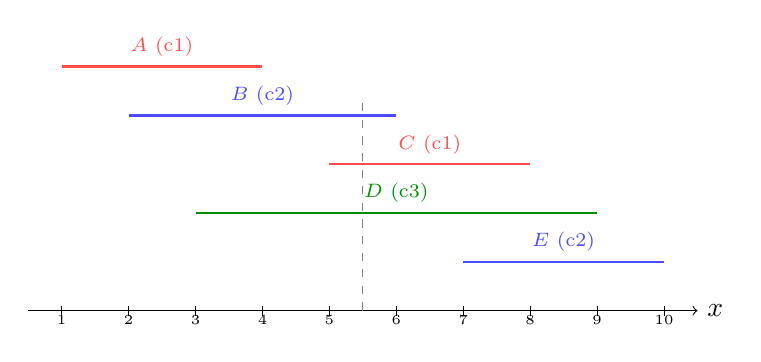
\begin{tikzpicture}[xscale=0.85,yscale=0.62]
  \draw[thick,red!70]   (1,5)--(4,5) node[midway,above,font=\scriptsize]{$A$ (c1)};
  \draw[thick,blue!70]  (2,4)--(6,4) node[midway,above,font=\scriptsize]{$B$ (c2)};
  \draw[thick,red!70]   (5,3)--(8,3) node[midway,above,font=\scriptsize]{$C$ (c1)};
  \draw[thick,green!55!black] (3,2)--(9,2) node[midway,above,font=\scriptsize]{$D$ (c3)};
  \draw[thick,blue!70]  (7,1)--(10,1) node[midway,above,font=\scriptsize]{$E$ (c2)};
  \draw[->] (0.5,0)--(10.5,0) node[right]{$x$};
  \foreach \x in {1,...,10} \draw (\x,-0.1)--(\x,0.1) node[below,font=\tiny]{\x};
  \draw[dashed,gray] (5.5,0)--(5.5,4.4);
\end{tikzpicture}
\end{center}
The dashed line at $x=5.5$ stabs $B,C,D$ -- three pairwise overlapping intervals,
the clique that forces three colors.
\end{labbox}

\begin{applicationbox}
\textbf{Interval scheduling / room assignment.} Tasks are intervals in time; two
tasks conflict iff they overlap; the minimum number of rooms (or machines) needed
is exactly $\chi$ of the interval graph, which equals the maximum number of tasks
live at any instant ($\omega$). The greedy ``assign each task to any free room,
sorted by start time'' is precisely the PEO coloring. This is why airport gate
assignment, conference room booking, and bandwidth allocation on a line all admit
clean optimal greedy solutions, while their two-dimensional cousins (which are not
interval graphs) become hard.
\end{applicationbox}

\section{The Cliff: Coloring Is NP-Hard}
\label{ch28:nphard}

Everything tractable in this chapter exploited special structure -- two colors,
bounded degree, an elimination ordering. Strip that away and coloring becomes one
of the canonical hard problems.

\begin{theorem}[Hardness of coloring]
\label{ch28:thm-nphard}
Deciding whether $\chi(\Gph)\le k$ is NP-complete for every fixed $k\ge 3$. In
particular \textsc{3-Coloring} is NP-complete. Computing $\chi(\Gph)$ exactly is
NP-hard, and unless $\mathsf{P}=\mathsf{NP}$ no polynomial algorithm approximates
$\chi(\Gph)$ within a factor $n^{1-\eps}$ for any $\eps>0$.
\end{theorem}

\begin{intuitionbox}
The chasm between $2$ and $3$ colors is the starkest phase transition in
algorithmic graph theory. Two-coloring is a single BFS; three-coloring is
NP-complete. Nothing continuous bridges them -- the difficulty does not grow with
$k$, it detonates the instant $k=3$. The reason is expressive power: with three
colors available you can build logical gadgets (a vertex's color encodes a Boolean
value, triangles enforce ``not equal,'' shared vertices propagate constraints) rich
enough to simulate any \textsc{3-SAT} formula.
\end{intuitionbox}

We sketch the gadget reduction to convey why $3$ is the magic threshold; the full
treatment lives in the NP-hardness chapter.

\begin{proof}[Proof idea: \textsc{3-SAT}\,$\le_p$\,\textsc{3-Coloring}]
Fix three palette colors and name them \textsf{T}, \textsf{F}, \textsf{N} (true,
false, neutral). Add a base triangle on three vertices named $T,F,N$ so the names
are pinned to actual colors. For each variable $x$ add two vertices $x,\bar x$
joined to each other and to $N$; this forces $\set{c(x),c(\bar x)}=\set{\textsf
T,\textsf F}$, i.e.\ a Boolean value. For each clause attach an ``OR gadget'' (a
small fixed graph on six vertices) wiring the three literal vertices to the base
triangle so that the gadget is $3$-colorable \emph{iff at least one literal is
colored} \textsf{T}. The whole graph is $3$-colorable iff the formula is
satisfiable. The construction is polynomial, so \textsc{3-Coloring} is NP-hard;
membership in NP is clear (a coloring is a checkable certificate).
\end{proof}

\begin{historybox}
\textsc{Chromatic Number} sits on Karp's original 1972 list of $21$ NP-complete
problems, and \textsc{3-Coloring} is the canonical hard restriction. The
inapproximability is far more recent: Feige and Kilian, and Hastad, showed in the
late 1990s, via the PCP theorem, that $\chi$ cannot be approximated within
$n^{1-\eps}$. Even the promise version -- given a graph that \emph{is}
$3$-colorable, find a coloring with few colors -- is brutal: the best known
polynomial algorithms still use roughly $n^{0.2}$ colors on a $3$-colorable graph,
and improving the exponent much is open and believed hard.
\end{historybox}

\begin{connectionbox}
Hardness does not mean helplessness. Three escape routes recur in this book.
\emph{Structure:} bounded-treewidth graphs admit exact coloring by dynamic
programming over a tree decomposition in time $\Oh^\star(k^{\tw})$ -- see the
treewidth and FPT chapters. \emph{Geometry/sparsity:} planar graphs are
$4$-colorable (and $5$-colorable easily), though $3$-colorability stays NP-complete
even for planar graphs of bounded degree. \emph{Relaxation:} the \emph{Lovasz theta
function} $\vartheta$, a semidefinite program computable in polynomial time, is
sandwiched between clique and chromatic data and seeds the celebrated
$\Oh(n^{0.2})$-coloring of $3$-colorable graphs via \emph{vector colorings}, taken
up in the approximation and spectral chapters.
\end{connectionbox}

\section{Register Allocation and Scheduling}
\label{ch28:applications}

\begin{applicationbox}
\textbf{Register allocation.} A compiler must map the unboundedly many
\emph{variables} of a program onto the few physical \emph{registers} of the CPU.
Two variables that are simultaneously \emph{live} -- both needed at some future
point -- cannot share a register. Build the \emph{interference graph}: one vertex
per variable, an edge between variables whose live ranges overlap. A proper
$k$-coloring is an assignment of variables to $k$ registers with no clash. So
register allocation \emph{is} graph coloring, with $k$ the number of machine
registers.

Chaitin's insight (1981) was to attack it with iterated greedy. Repeatedly remove a
vertex of degree $<k$ (it can always be colored later, since fewer than $k$
neighbors leave a free register) and push it on a stack -- this is exactly building
a degeneracy-style ordering. If at some point every remaining vertex has degree
$\ge k$, \emph{spill} one variable to memory (delete it from the graph and reload it
around its uses), then continue. Pop the stack and color greedily. When live ranges
are computed on a structured (reducible) control-flow graph in SSA form, the
interference graph is chordal, and then this is the \emph{optimal} chordal coloring
of Theorem~\ref{ch28:thm-chordal-color} -- which is why SSA-based allocators can drop
spilling heuristics and color provably optimally in linear time. The $\Delta+1$
greedy bound, the degeneracy ordering, and the chordal theorem of this chapter are
not analogies here; they are the literal algorithm running in your compiler.
\end{applicationbox}

\begin{applicationbox}
\textbf{Timetabling and frequency assignment.} Exams that share a student cannot run
in the same slot: vertices are exams, edges are shared students, colors are time
slots, and $\chi$ is the shortest exam timetable. Mobile transmitters too close
together cannot reuse a frequency: vertices are transmitters, edges are interfering
pairs, colors are frequencies. Both are coloring, both are NP-hard in general, and
both are attacked in practice by exactly the toolkit here -- greedy on a good
(degeneracy or saturation-degree ``DSATUR'') order, Brooks-style one-color savings
when no clique forces the worst case, and chordal/interval optimality when the
conflict structure happens to be an interval graph (e.g.\ a single linear corridor
of transmitters).
\end{applicationbox}

\begin{complexitybox}
\textbf{Chapter cost summary.}
\begin{center}
\begin{tabular}{lll}
\toprule
Task & Method & Cost / guarantee\\
\midrule
Proper coloring (any) & greedy, fixed order & $\Oh(n+m)$, $\le\Delta+1$ colors\\
Best greedy bound & degeneracy ordering & $\Oh(n+m)$, $\le\degen+1$ colors\\
$2$-colorability & BFS & $\Oh(n+m)$, exact + certificate\\
$\le\Delta$ colors & Brooks (non-clique, non-odd-cycle) & polynomial, exact bound\\
Edge coloring & Vizing fans + Kempe chains & $\Oh(nm)$, $\le\Delta+1$ colors\\
Chordal / interval & PEO via Lex-BFS, then greedy & $\Oh(n+m)$, \emph{optimal}\\
$\chi$ exactly, general & (NP-hard) DP on treewidth & $\Oh^\star(k^{\tw})$\\
$\chi\le k$, $k\ge 3$ & --- & NP-complete\\
\bottomrule
\end{tabular}
\end{center}
\end{complexitybox}

\begin{connectionbox}
\textbf{What This Unlocked:}
Graph coloring provided the mathematical language for discrete conflict resolution.
Brooks's and Vizing's theorems established tight upper bounds based on local maximum degrees,
while Lex-BFS and Perfect Elimination Orderings unlocked exact linear-time coloring for
chordal and interval graphs. Gregory Chaitin (1981) applied graph coloring to compiler
register allocation, turning compiler code generation from ad-hoc heuristics into an exact,
principled graph algorithm.

\textbf{Honest Downsides and Limitations:}
\begin{itemize}
  \item \emph{Hardness of approximation:} Deciding whether a planar graph of maximum degree 4
        is 3-colorable is NP-complete (Garey, Johnson, Stockmeyer 1976). On general graphs,
        coloring cannot be approximated within $n^{1-\eps}$ for any $\eps > 0$ unless
        $\mathrm{P} = \mathrm{NP}$ (Zuckerman 2007).
  \item \emph{Order-sensitivity of greedy heuristics:} As shown in Exercise~\ref{ch28:ex-crown},
        a bad ordering can force the greedy algorithm to use $n/2$ colors on a graph with
        $\chi(\Gph) = 2$.
  \item \emph{Local vs. global gap:} A graph can have no triangles ($\omega(\Gph) = 2$) yet
        have an arbitrarily large chromatic number $\chi(\Gph)$ (Mycielski's construction),
        showing that local clique checks cannot detect global coloring obstructions.
\end{itemize}

\textbf{Where We Go Next:}
A proper coloring partitions the vertex set into independent sets. How do we find the
largest possible independent set, or dually, the largest clique? In \textbf{Chapter~29
(Independent Sets, Cliques, and Vertex Covers)}, we examine exact algorithms and the
Bron--Kerbosch pivoting algorithm.
Then, for which broad family of graphs is the chromatic number $\chi(H)$ always equal to the
clique number $\omega(H)$ on every induced subgraph? That is the pristine subject of
\textbf{Chapter~30 (Perfect Graphs)}.
\end{connectionbox}

\section{Exercises}
\label{ch28:exercises}

\begin{exercise}[Greedy adversary]
\label{ch28:ex-crown}
The \emph{crown graph} $S_n^0$ is $K_{n,n}$ with a perfect matching removed. Prove
$\chi(S_n^0)=2$, then exhibit a vertex order on which Algorithm~\ref{ch28:alg-greedy} uses
$n$ colors. Conclude that the gap between greedy's worst order and $\chi$ is
unbounded.
\end{exercise}

\begin{exercise}[Degeneracy versus max degree]
\label{ch28:ex-degen}
Show $\degen(\Gph)\le\Delta(\Gph)$ always, and construct, for each $d$, a graph with
$\degen=d$ but $\Delta$ arbitrarily large. Then prove every simple planar graph is
$5$-degenerate (use that it has $\le 3n-6$ edges, so average degree $<6$), and
deduce the six-color theorem for planar graphs.
\end{exercise}

\begin{exercise}[Odd-cycle certificate]
\label{ch28:ex-oddcycle}
Modify Algorithm~\ref{ch28:alg-twocolor} so that, on failure, it outputs an actual odd cycle
(not merely the conflicting edge). Prove your reconstruction is correct and runs in
$\Oh(n+m)$. Why does this certificate constitute a co-NP-style proof of
non-$2$-colorability?
\end{exercise}

\begin{exercise}[Brooks by hand]
\label{ch28:ex-brooks}
Take the $3$-cube graph $Q_3$ ($\Delta=3$, $3$-regular, bipartite). Brooks
guarantees $\chi\le 3$; bipartiteness guarantees $\chi=2$. Reconcile these and
exhibit the $2$-coloring. Then find a connected $3$-regular graph that is \emph{not}
bipartite and color it with $3$ colors using the ordering trick from the proof of
Theorem~\ref{ch28:thm-brooks}.
\end{exercise}

\begin{exercise}[Vizing classes]
\label{ch28:ex-vizing}
Compute $\chi'$ for $K_4$, $K_5$, the Petersen graph, and $C_5$. Which are Class~1
($\chi'=\Delta$) and which Class~2 ($\chi'=\Delta+1$)? Prove that every connected
$\Delta$-regular graph with an \emph{odd} number of vertices is Class~2. (Hint: a
color class is a matching, which saturates an even number of vertices.)
\end{exercise}

\begin{exercise}[Line graphs and edge coloring]
\label{ch28:ex-linegraph}
Prove $\chi'(\Gph)=\chi(L(\Gph))$ where $L$ is the line graph. Using Vizing, deduce
$\chi(L(\Gph))\le\Delta(\Gph)+1$. Give an example where $L(\Gph)$ is \emph{not}
perfect, showing edge coloring's good behavior is special to line graphs and not a
consequence of perfection.
\end{exercise}

\begin{exercise}[Simplicial vertices]
\label{ch28:ex-simplicial}
Prove that every chordal graph with at least two vertices has at least two
simplicial vertices, and that if it is not complete the two can be chosen
non-adjacent. Use this to give an alternative inductive proof of
Theorem~\ref{ch28:thm-chordal-color} that does not invoke Lex-BFS.
\end{exercise}

\begin{exercise}[Interval coloring is room scheduling]
\label{ch28:ex-interval}
Given $n$ intervals, design an $\Oh(n\log n)$ algorithm that assigns each a color
(room) using exactly the maximum overlap depth $\omega$ many colors. Prove
optimality by exhibiting a point stabbed by $\omega$ intervals. Where does the
argument break if the ``intervals'' are arcs on a circle rather than segments on a
line?
\end{exercise}

\begin{exercise}[Mycielski's triangle-free tower]
\label{ch28:ex-mycielski}
The Mycielskian $M(\Gph)$ adds, for each vertex $v$, a twin $v'$ joined to $v$'s
neighbors, plus one apex $w$ joined to all twins. Prove $M(\Gph)$ is triangle-free
if $\Gph$ is, and that $\chi(M(\Gph))=\chi(\Gph)+1$. Starting from $K_2$, build a
triangle-free graph with $\chi=4$ and report its vertex count.
\end{exercise}

\begin{exercise}[3-coloring gadget]
\label{ch28:ex-gadget}
Design the OR gadget used in Theorem~\ref{ch28:thm-nphard}: a small graph attached to the
base triangle and to three literal vertices that is $3$-colorable iff at least one
literal is colored \textsf{T}. Verify your gadget by checking all $8$ truth
assignments of the literals. Conclude the reduction is polynomial in formula size.
\end{exercise}

\begin{exercise}[Register allocation with spilling]
\label{ch28:ex-regalloc}
Implement Chaitin-style allocation: given an interference graph and $k$ registers,
repeatedly remove a vertex of degree $<k$ (stack it); if stuck, spill a
highest-degree vertex; finally pop and color. Prove that if the interference graph
is chordal, the ``stuck'' case never arises for $k=\omega$, so no spilling is needed
and the allocation is optimal. Connect this to Theorem~\ref{ch28:thm-chordal-color}.
\end{exercise}
